\section{Введение}\label{sec:intro}
\subsection{Языковые модели в~задачах программной инженерии}
Большие языковые модели помогают писать код, находить ошибки и~готовить исправления. Для работы им нужны текстовый запрос и~контекст: условие задачи, исходный код, документация и~другие доступные сведения. Модель предлагает программу. Чтобы проверить её, запускают код на тестовых данных и~сопоставляют полученный результат с~ожидаемым.

Работу модели можно разделить на три действия. Сначала она анализирует требования и~составляет план, затем пишет код, после чего ищет недостатки и~исправляет их. Последнее действие далее называем \emph{рецензированием}. В~запросе эти действия поручаются планировщику, исполнителю и~рецензенту. Здесь \emph{роль} означает инструкцию модели выполнить определённую часть работы.

В~этой статье \emph{вызов} --- одно обращение к~LLM, при котором система передаёт запрос и~получает ответ. При \emph{интроспективном вызове}, обозначенном далее как SR, модели одним INoT-промптом предлагают последовательно спланировать решение, написать код и~проверить его в~рамках этого вызова. Introspection of Thought (INoT) --- метод промптинга, в~котором действия нескольких ролей задаются в~одном вызове~\cite{sun2025inot}. В~нашем варианте один запрос задаёт роли планировщика, исполнителя и~рецензента, а~также порядок их работы. Наблюдать можно инструкции и~ответ модели, а~разделение действий в~её скрытых рассуждениях остаётся неизвестным.

При \emph{последовательных вызовах} выполняются три отдельных обращения к~LLM. Первый запрос поручает составить план. Второй получает этот план и~поручает написать код. Третий получает предыдущие ответы и~поручает проверить и~исправить программу. Каждый вызов также получает полный исходный контекст задачи. Условие с~названиями ролей обозначается \MultiCallRole{}. В~сравниваемых условиях используется одна и~та же модель.

\subsection{Повторная передача контекста и~затраты}
Длину текста измеряют в~\emph{токенах}. Токен --- единица, на которую модель разбивает текст: слово, часть слова или знак. Расход складывается из входных токенов, переданных модели, и~выходных токенов, созданных ею. При последовательных вызовах одинаковая часть контекста передаётся трижды. К~ней добавляются промежуточные ответы. Рисунок~\ref{fig:context-flow} показывает, откуда возникает повторная передача.

\begin{figure}[htbp]
\centering
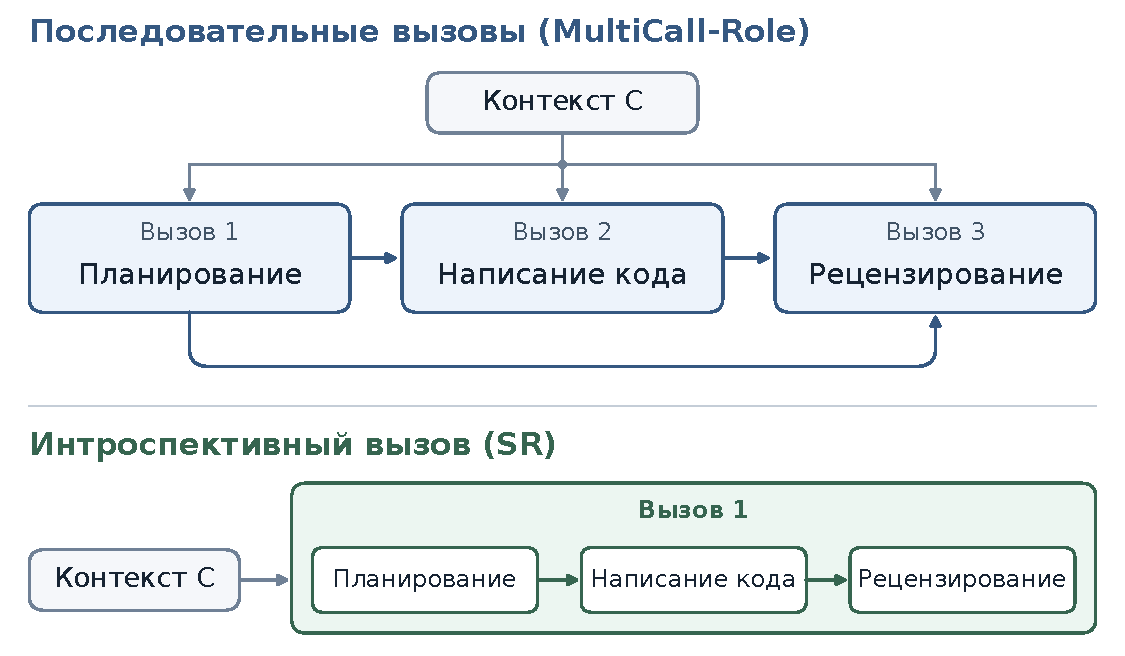
\includegraphics[width=\textwidth]{figures/context-flow.pdf}
\caption{Передача исходного контекста $C$ при трёх последовательных вызовах и~одном интроспективном. Вверху стрелки между вызовами показывают, куда передаются ответы. Внизу стрелки внутри общего блока показывают порядок действий, заданный одним запросом.}
\label{fig:context-flow}
\end{figure}
\FloatBarrier

Например, если общий контекст содержит 4\,000 токенов, три вызова получают в~сумме 12\,000 входных токенов контекста, а~интроспективный вызов получает 4\,000. Разница составляет 8\,000 токенов. Означает ли это, что с~увеличением общего контекста объединять вызовы становится выгоднее? Если остальные составляющие одинаковы, каждый дополнительный токен общего контекста увеличивает разницу на два входных токена. Чтобы оценить весь расход и~его стоимость, нужно учесть также длину инструкций и~ответов, подготовку контекста, кэширование и~возможные вызовы для исправления кода (раздел~\ref{sec:analysis}).

Что требует меньше энергии при решении одной задачи --- один вызов со всеми этапами или три вызова, каждый с~одним этапом и~повторной передачей контекста? Для ответа нужны измерения вычислительной нагрузки и~энергии всех операций, включая самую ресурсоёмкую. В~этой работе измеряется расход токенов и~оценивается их тарифная стоимость. Энергопотребление оборудования в~эти измерения не входит.

В~аналитической части сравниваемый вариант последовательных вызовов обозначен как Classical-MAS, а~в~эксперименте как \MultiCallRole{}. Каждый его вызов получает полный контекст. В~других схемах взаимодействия ролей передача данных может быть устроена иначе. Интроспективный вызов может дать более длинный ответ, рецензирование может пропустить ошибку, а~исправление может потребовать нового обращения к~модели. Поэтому экономию оцениваем вместе с~долей программ, успешно прошедших независимую проверку.

\subsection{Цель, вопросы и~задачи исследования}
Цель работы --- определить, при каких условиях один интроспективный вызов снижает расход токенов и~расчётную стоимость генерации кода по сравнению с~тремя последовательными вызовами, и~оценить изменение качества относительно этого базового варианта.

За меру качества принимаем долю программ, прошедших все тесты задачи. Обозначим эту долю в~процентах через $p_{\mathrm{SR}}$ для интроспективного вызова и~$p_{\mathrm{base}}$ для базового последовательного варианта. Разность $\Delta_Q=p_{\mathrm{SR}}-p_{\mathrm{base}}$ измеряется в~процентных пунктах. Если допустимое снижение качества заранее задано как $\delta\geq 0$ п.п., целевая граница для разности равна $-\delta$. В~проведённых сериях оцениваем разность долей и~её неопределённость. Значение $\delta$ требуется для отдельной проверки не меньшей эффективности (раздел~\ref{sec:analysis}).

Основной вопрос работы состоит в~том, \emph{когда объединение этапов снижает расход и~расчётную стоимость всех вызовов на задачу и~как при этом меняется доля успешных решений относительно базового варианта}. Расход рассматриваем с~точки зрения пользователя, который обращается к~модели через API или по подписке. В~обоих случаях число токенов характеризует объём работы с~моделью. Тарифная оценка показывает стоимость такого объёма при оплате по API. Фактическая плата за подписку определяется её условиями, а~оборудование и~энергозатраты поставщика обсуждаются отдельно (раздел~\ref{sec:limits}).

Для сравнения сформулированы четыре вопроса.
\begin{enumerate}
\item \textbf{RQ1.} Как меняется доля программ, успешно прошедших независимую проверку на тестах BigCodeBench, при переходе от трёх последовательных вызовов к~одному интроспективному?
\item \textbf{RQ2.} Как при таком переходе меняются суммарный расход входных и~выходных токенов и~расчётная стоимость обращений к~модели и~при каких условиях объединение этапов даёт экономию с~учётом подготовки контекста, ответов и~возможных исправлений?
\item \textbf{RQ3.} Как интроспективный вызов соотносится по доле программ, прошедших одни и~те же независимые тесты, с~прямым запросом и~с~многошаговой процедурой, где модель отдельно вызывается в~ролях аналитика, разработчика и~тестировщика, и~как различается расчётная стоимость интроспективного и~многошагового способов?
\item \textbf{RQ4.} Как меняются доля успешных программ, расход токенов, расчётная стоимость и~время решения, если контроллер для каждой задачи выбирает между одним и~тремя вызовами по заранее заданному требованию к~разделению работы?
\end{enumerate}

В~качестве многошагового варианта в~RQ3 используется Self-Collaboration Code Generation (SCC)~\cite{dong2023selfcollaboration}. В~этой процедуре одна модель по очереди выполняет роли аналитика, разработчика и~тестировщика. Контроллер запускает код на примерах тестировщика и~может запросить исправление. Поэтому сравнение с~SCC охватывает всю процедуру, включая внутренние проверки. Качество готового кода в~сравнении с~SCC оценивается по независимым тестам BigCodeBench (приложение~\ref{subsec:scc}).

\Needspace{7\baselineskip}
Исследование включает пять задач.
\begin{enumerate}
\item Зафиксировать содержание запросов, действия модели, формат итогового кода и~единый критерий проверки, чтобы сравнение способов вызова можно было воспроизвести на одних и~тех же задачах.
\item Вывести условия, при которых процедура с~интроспективным вызовом требует меньше токенов, чем процедура с~последовательными вызовами, с~учётом подготовки контекста и~возможных исправлений.
\item Сопоставить способы организации вызовов на одних и~тех же задачах. Добавить варианты без названий ролей, чтобы проверить, связано ли различие с~самим разделением работы или с~формулировкой инструкции.
\item Оценить качество кода по доле программ, прошедших тесты, и~проверить, как на вывод влияют разброс результатов повторных генераций и~пропуски.
\item Сравнить расход токенов и~расчётную стоимость с~учётом промежуточных ответов. Если есть незавершённые запуски, учесть и~их известные расходы.
\end{enumerate}

\emph{Доверительный интервал} показывает точность оценки разницы долей успеха. В~главном сравнении $A$ --- один интроспективный вызов SR, а~$B$ --- три последовательных вызова \MultiCallRole{}. Результат $Y_{imr}$ равен 1, если программа в~прогоне $r$ способа $m$ на задаче $i$ прошла тесты, и~0 в~случае неуспеха. Сопоставляем доли успеха за три прогона каждого способа на задачу. Усредняем разности по $n$ задачам с~шестью известными исходами и~выражаем оценку в~процентных пунктах.
\begin{formulakey}
\[
 d_i=\frac{1}{3}\sum_{r=1}^{3}(Y_{iAr}-Y_{iBr}),
 \qquad \widehat{\Delta}_Q=\frac{100}{n}\sum_{i=1}^{n}d_i.
\]
\begin{symbols}
\sym{i,\ r}{номер задачи и~номер одного из трёх прогонов}
\sym{A,\ B}{сравниваемые способы, один и~три вызова соответственно}
\sym{Y_{iAr},\,Y_{iBr}}{результаты тестов двух программ в~этом повторе, 1 при успехе и~0 при неуспехе}
\sym{d_i}{разность долей успеха на одной задаче}
\sym{n,\ \widehat{\Delta}_Q}{число задач с~полными данными и~средняя разность по ним в~процентных пунктах}
\end{symbols}
\end{formulakey}
Повторно набираем из исходной выборки 10\,000 наборов по $n$ задач. Это \emph{парный бутстрэп}~\cite{efron1986bootstrap}. В~один набор задача может попасть несколько раз. Для неё каждый раз берём разность $d_i$, рассчитанную по всем шести прогонам. Если у~$A$ на задаче прошли тесты две программы, а~у~$B$ одна, берём $d_i=2/3-1/3$. Для каждого набора пересчитываем среднюю разность. Границы интервала отсекают по 2,5\% самых низких и~самых высоких оценок. При повторении исследования примерно 95\% таких интервалов охватили бы разницу долей успеха, которую в~среднем даёт эксперимент при тех же настройках и~отборе задач. Это свойство зависит от предпосылок метода.

В~таблице~\ref{tab:scale-contrasts} четыре разности долей успеха. Сравниваем один вызов с~тремя отдельно для запросов с~названиями ролей и~для запросов с~номерами этапов. Также сравниваем названия ролей с~номерами этапов при одном и~при трёх вызовах. Чтобы охватить все четыре разности одновременно примерно с~95\%-й надёжностью, по поправке Бонферрони~\cite{nistbonferroni} строим каждый интервал Стьюдента с~уровнем $1-0{,}05/4=98{,}75\%$ (таблица~\ref{tab:precision}).

\Needspace{6\baselineskip}
Основную оценку считаем по задачам с~полными результатами. Отдельно проверяем, могли ли пропуски изменить вывод на всей тысяче задач. Для этого подставляем крайние возможные исходы вместо неизвестных. Даже самый неблагоприятный для одного вызова вариант оставляет разность положительной (раздел~\ref{subsec:missing-outcomes}).

\subsection{Интроспективный вызов и~основные результаты}
В~основном эксперименте при SR модель получала исходный контекст и~инструкции для всех трёх этапов одним запросом. На один прогон SR приходилось одно обращение к~модели. После генерации код запускал отдельный оценщик BigCodeBench. Внешние тесты давали общий критерий качества для всех способов и~выполнялись без обращения к~LLM.

В~формальном описании Hybrid-INoT из раздела~\ref{sec:method} предусмотрен дополнительный режим. Если код проваливает доступные во время работы тесты, можно передать сообщение об~ошибке модели для исправления. Такое исправление требует второго вызова, расход которого входит в~общий бюджет. В~сравнении на BigCodeBench итоговые тесты запускались после последнего ответа модели. В~разделе~\ref{sec:analysis} выведено условие экономии токенов для RQ2 с~учётом подготовки контекста, ответов и~возможных исправлений.

BigCodeBench~\cite{zhuo2024bigcodebench} содержит задачи на написание функций Python и~автоматические тесты к~ним. Две основные серии сравнивают число вызовов и~наличие названий ролей на 200 и~1\,000 задачах этого набора. В~отдельной серии на 80 задачах сравнили названия ролей и~номера этапов при одинаковых требованиях к~планированию, написанию и~проверке кода. Два способа оформления позволяют проверить это различие при записи этапов по строкам и~в~одном абзаце. Полные запросы приведены в~приложениях~\ref{app:prompt-lines} и~\ref{app:prompt-paragraph}. Проведено также сравнение с~SCC. Подготовительная серия на 40 задачах использовалась для отладки извлечения кода из ответа и~его запуска на автоматических тестах. Устройство серий и~пересечения выборок описаны в~разделе~\ref{sec:eval}.

В~расширенной серии полные данные о~расходе обоих способов доступны на 986 задачах. У~15 из них среда тестирования не прошла контроль на эталонной и~заведомо неверной программах. Расходы на этих задачах входят в~ресурсное сравнение. Для совместного сравнения использована 971 задача с~полными результатами тестов и~данными о~расходе. На этих задачах доля успехов при одном вызове выше на 2,13 процентного пункта, а~суммарная расчётная стоимость на 64,1\% ниже, чем при трёх последовательных. В~сумму входят и~расходы на программы, провалившие тесты (таблица~\ref{tab:scale-quality-cost}).

Для совместной оценки делим суммарную расчётную стоимость каждого способа на число программ, прошедших тесты. На общей выборке эта стоимость на одну успешную программу была у~интроспективного вызова ниже на 65,5\%.

В~отдельной локальной серии для RQ4 сам контроллер выбирает число вызовов по требованию к~сессии рецензента. В~этом сравнении время измерено от выбора режима до получения результата тестирования (раздел~\ref{subsec:route-pilot}).

\section{Связанные работы и~отличие предлагаемого подхода}\label{sec:related}
\subsection{Промежуточные рассуждения и~исправление ответа}
Wei и~соавторы~\cite{wei2022cot} исследовали Chain-of-Thought. Модель получает примеры, в~которых перед ответом записаны промежуточные шаги решения. На изученных арифметических, логических и~символьных задачах такие примеры повышали долю правильных ответов у~ряда крупных моделей. Это показало, что способ задания рассуждения может влиять на результат, хотя величина эффекта зависит от модели и~задачи.

В~Self-Refine Madaan и~соавторы~\cite{madaan2023selfrefine} используют одну модель для получения ответа, подготовки замечаний и~исправления. Эти операции выполняются через последовательные обращения к~модели. Reflexion Shinn и~соавторов~\cite{shinn2023reflexion} добавляет память о~прошлых ошибках: текстовую обратную связь сохраняют и~используют в~следующих попытках. Такая обратная связь может поступать как от модели, так и~из внешней среды.

ReAct Yao и~соавторов~\cite{yao2022react} чередует рассуждение с~действиями, например поиском информации. Полученное наблюдение помогает выбрать следующий шаг. Sun и~Zeng~\cite{sun2025inot} в~Introspection of Thought (INoT) задают диалог и~самопроверку с~помощью инструкции, похожей на программу. Hybrid-INoT развивает идею организации ролевых действий в~одном обращении к~модели и~дополняет её внешней проверкой кода. В~основном эксперименте изучается только объединение заданных действий. Прямое превосходство над оригинальным INoT этим сравнением не проверяется.

Turpin и~соавторы~\cite{turpin2023unfaithful} показали, что записанная цепочка рассуждений может не отражать причин ответа модели. Поэтому в~Hybrid-INoT план и~замечания рецензента служат рабочим текстом. Их полезность оценивается по итоговой программе, расходу ресурсов и~результатам независимых тестов.

\subsection{Отдельные агенты и~задачи программирования}
В~мультиагентных системах работу распределяют между взаимодействующими участниками~\cite{weiss1999,wooldridge2009}. MetaGPT~\cite{hong2023metagpt} и~ChatDev~\cite{qian2023chatdev} применяют такой подход к~разработке программ. Участники выполняют разные функции и~передают друг другу результаты. Набор инструментов и~состав контекста определяются реализацией каждой системы.

Обзоры и~исследования масштабирования обсуждают трудности согласования работы агентов~\cite{guo2024survey,qian2024scaling}. Одна из них --- расход на повторную передачу контекста и~промежуточных сообщений. Число сообщений зависит от порядка взаимодействия. При обмене между каждой парой ролей оно может расти квадратично с~числом ролей. В~последовательной цепочке сообщений существенно меньше. Поэтому затраты нужно считать для конкретного процесса.

Self-Collaboration Code Generation (SCC)~\cite{dong2023selfcollaboration} близок к~исследуемой последовательности: аналитик, разработчик и~тестировщик взаимодействуют через отдельные обращения к~модели. Для сравнения использован авторский код SCC с~изменёнными интерфейсом вызова и~числом итераций. Эти изменения описаны в~приложении~\ref{subsec:scc}. В~отличие от основного сравнения одного и~трёх вызовов, серия с~SCC оценивает процесс целиком, включая его внутренние проверки.

Для оценки кода применяются задачи разного масштаба. HumanEval~\cite{chen2021humaneval} содержит задания на написание отдельных функций. SWE-bench~\cite{jimenez2023swebench} проверяет исправления в~реальных репозиториях, а~SWE-agent~\cite{yang2024sweagent} исследует влияние интерфейса доступа к~файлам и~инструментам на их решение. В~нашей работе выбран BigCodeBench~\cite{zhuo2024bigcodebench}: задачи на создание функций Python с~использованием библиотек и~подробных требований. Его тесты позволяют сравнить программы в~одинаковых условиях. Измерения в~этой серии относятся к~отдельным функциям Python.

\subsection{Сжатие контекста и~внешние проверки}
LongLLMLingua~\cite{jiang2023longllmlingua} и~LLMLingua-2~\cite{pan2024llmlingua2} сокращают входной текст, стараясь сохранить нужную для ответа информацию. Jia и~соавторы~\cite{jia2026compression} исследуют сжатие кода при исправлении задач из репозиториев. В~основном сравнении мы передаём полный исходный контекст. Оценка методов его сжатия при передаче между вызовами выходит за рамки исследования.

Внешние инструменты проверяют программу независимо от того, насколько убедительно модель описывает своё решение. Тест выполняет код на заданных входных данных и~сверяет полученные выходные данные с~ожидаемыми. Статический анализ исследует свойства программы без её запуска. Компилятор обнаруживает нарушения правил языка и~часть несовместимостей интерфейсов. CoCoGen~\cite{bi2024cocogen} использует обратную связь компилятора для уточнения кода с~учётом проекта. Su и~McMillan~\cite{su2025static} исследуют ограничения самих языковых моделей в~задачах статического анализа. Оценщик отмечает решение как успешное, если программа проходит все выбранные тесты.
